% Created 2014-09-11 Thu 17:07
\documentclass[table,smaller]{beamer}
\usepackage[utf8]{inputenc}
\usepackage[T1]{fontenc}
\usepackage{fixltx2e}
\usepackage{graphicx}
\usepackage{longtable}
\usepackage{float}
\usepackage{wrapfig}
\usepackage{rotating}
\usepackage[normalem]{ulem}
\usepackage{amsmath}
\usepackage{textcomp}
\usepackage{marvosym}
\usepackage{wasysym}
\usepackage{amssymb}
\usepackage{hyperref}
\tolerance=1000
\usepackage{tikz}
\usepackage{minted}
\usepackage{fancyvrb}
\usemintedstyle{perldoc}
\definecolor{lightgray}{gray}{0.96}
\setlength{\tabcolsep}{1ex}
\usetheme{Warsaw}
\useoutertheme{infolines}
\setbeamercolor{block body}{bg=lightgray}
\titlegraphic{
\includegraphics[width=.75\textwidth]{images/IQSSNewLogo.pdf}}
\setbeamersize{text margin left=2em,text margin right=2em}
\AtBeginSection[]{\begin{frame}<beamer>\frametitle{Topic}\tableofcontents[currentsection]\end{frame}}
\usetheme{default}
\author{}
\date{}
\title{Regression Models in R}
\hypersetup{
  pdfkeywords={},
  pdfsubject={},
  pdfcreator={Emacs 24.3.1 (Org mode 8.2.7c)}}
\begin{document}

\maketitle
\begin{frame}{Outline}
\tableofcontents
\end{frame}



\section{Introduction}
\label{sec-1}

\begin{frame}[label=sec-1-1]{Workshop description}
\begin{itemize}
\item This is an intermediate/advanced R course
\item Appropriate for those with basic knowledge of R
\item This is not a statistics course!
\item Learning objectives:
\begin{itemize}
\item Learn the R formula interface
\item Specify factor contrasts to test specific hypotheses
\item Perform model comparisons
\item Run and interpret variety of regression models in R
\end{itemize}
\end{itemize}
\end{frame}

\begin{frame}[label=sec-1-2]{Materials and Setup}
Lab computer users: Log in using the user name and password on the board to your left.

Everyone should have R installed --if not:

\begin{itemize}
\item Open a web browser and go to \url{http://cran.r-project.org} and download and install it
\item Also helpful to install RStudo (download from \url{http://rstudio.com})
\end{itemize}

Materials for this workshop include slides, example data sets, and example code.

\begin{itemize}
\item Download materials from \url{http://tutorials.iq.harvard.edu/R/Rstatistics.zip}
\item Extract materials from RStatistics.zip (on lab machines \emph{right-click -> WinZip -> Extract to here}) and move to your desktop.
\end{itemize}
\end{frame}

\begin{frame}[fragile,label=sec-1-3]{Launch RStudio}
 \begin{itemize}
\item Open the RStudio program from the Windows start menu

\item Open up today's R script
\begin{itemize}
\item In RStudio, Go to \alert{File => Open Script}
\item Locate and open the \texttt{Rstatistics.R} script in the Rstatistics folder on your desktop
\end{itemize}

\item Go to \alert{Tools => Set working directory => To source file location} (more on the working directory later)
\item I encourage you to add your own notes to this file!
\end{itemize}
\end{frame}


\begin{frame}[fragile,label=sec-1-4]{Set working directory}
 It is often helpful to start your R session by setting your working directory so you don't have to type the full path names to your data and other files

\vspace{-.5em}
\begin{columns}
\column{.95\linewidth}
\begin{block}{}
\begin{minted}[linenos=false, fontsize=\footnotesize]{rconsole}
> # set the working directory
> # setwd("~/Desktop/Rstatistics")
> # setwd("C:/Users/dataclass/Desktop/Rstatistics")
>
\end{minted}
\end{block}
\end{columns}
\vspace{.5em}

You might also start by listing the files in your working directory
\vspace{-.5em}
\begin{columns}
\column{.95\linewidth}
\begin{block}{}
\begin{minted}[linenos=false, fontsize=\footnotesize]{rconsole}
> getwd() # where am I?
[1] "/home/izahn/Documents/Work/IQSS/Classes/IQSS_Stats_Workshops/R/Rstatistics"
> list.files("dataSets") # files in the dataSets folder
[1] "Exam.rds"          "NatHealth2008MI"   "NatHealth2011.rds"
[4] "states.dta"        "states.rds"       
>
\end{minted}
\end{block}
\end{columns}
\vspace{.5em}
\end{frame}

\begin{frame}[fragile,label=sec-1-5]{Load the states data}
 The \emph{states.dta} data comes from \url{http://anawida.de/teach/SS14/anawida/4.linReg/data/states.dta.txt} and appears to have originally appeared in \emph{Statistics with Stata} by Lawrence C. Hamilton.
\vspace{-.5em}
\begin{columns}
\column{.95\linewidth}
\begin{block}{}
\begin{minted}[linenos=false, fontsize=\footnotesize]{rconsole}
> # read the states data
> states.data <- readRDS("dataSets/states.rds") 
> #get labels
> states.info <- data.frame(attributes(states.data)[c("names", "var.labels")])
> #look at last few labels
> tail(states.info, 8)
     names                      var.labels
14    csat        Mean composite SAT score
15    vsat           Mean verbal SAT score
16    msat             Mean math SAT score
17 percent       % HS graduates taking SAT
18 expense Per pupil expenditures prim&sec
19  income Median household income, $1,000
20    high             % adults HS diploma
21 college         % adults college degree
>
\end{minted}
\end{block}
\end{columns}
\vspace{.5em}
\end{frame}


\section{Linear regression}
\label{sec-2}

\begin{frame}[fragile,label=sec-2-1]{Examine the data before fitting models}
 Start by examining the data to check for problems.

\vspace{-.5em}
\begin{columns}
\column{.95\linewidth}
\begin{block}{}
\begin{minted}[linenos=false, fontsize=\footnotesize]{rconsole}
> # summary of expense and csat columns, all rows
> sts.ex.sat <- subset(states.data, select = c("expense", "csat"))
> summary(sts.ex.sat)
    expense          csat     
 Min.   :2960   Min.   : 832  
 1st Qu.:4352   1st Qu.: 888  
 Median :5000   Median : 926  
 Mean   :5236   Mean   : 944  
 3rd Qu.:5794   3rd Qu.: 997  
 Max.   :9259   Max.   :1093  
> # correlation between expense and csat
> cor(sts.ex.sat) 
        expense   csat
expense   1.000 -0.466
csat     -0.466  1.000
>
\end{minted}
\end{block}
\end{columns}
\vspace{.5em}
\end{frame}

\begin{frame}[fragile,label=sec-2-2]{Plot the data before fitting models}
 Plot the data to look for multivariate outliers, non-linear relationships etc.

\begin{columns} \column{.9\textwidth} \begin{block}{}
\begin{minted}[fontsize=\scriptsize]{r}
# scatter plot of expense vs csat
plot(sts.ex.sat)
\end{minted}

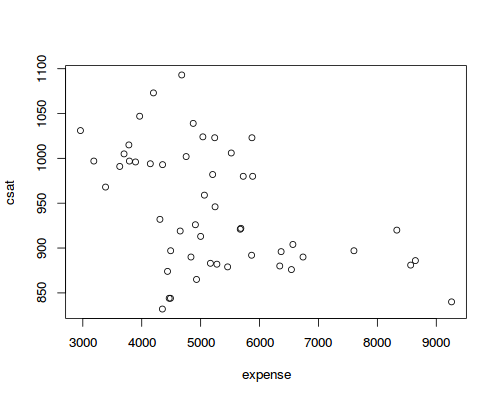
\includegraphics[width=2.5in]{images/statesCorr1.png}


\end{block} \end{columns}
\end{frame}

\begin{frame}[fragile,label=sec-2-3]{Linear regression example}
 \begin{itemize}
\item Linear regression models can be fit with the \texttt{lm()} function
\item For example, we can use \texttt{lm} to predict SAT scores based on per-pupal expenditures:
\end{itemize}

\vspace{-.5em}
\begin{columns}
\column{.95\linewidth}
\begin{block}{}
\begin{minted}[linenos=false, fontsize=\footnotesize]{rconsole}
> # Fit our regression model
> sat.mod <- lm(csat ~ expense, # regression formula
+               data=states.data) # data set
> # Summarize and print the results
> summary(sat.mod) # show regression coefficients table

Call:
lm(formula = csat ~ expense, data = states.data)

Residuals:
    Min      1Q  Median      3Q     Max 
-131.81  -38.08    5.61   37.85  136.50 

Coefficients:
              Estimate Std. Error t value Pr(>|t|)
(Intercept) 1060.73244   32.70090   32.44  < 2e-16
expense       -0.02228    0.00604   -3.69  0.00056

Residual standard error: 59.8 on 49 degrees of freedom
Multiple R-squared:  0.217,	Adjusted R-squared:  0.201 
F-statistic: 13.6 on 1 and 49 DF,  p-value: 0.000563

>
\end{minted}
\end{block}
\end{columns}
\vspace{.5em}
\end{frame}

\begin{frame}[fragile,label=sec-2-4]{Why is the association between expense and SAT scores \emph{negative}?}
 Many people find it surprising that the per-capita expenditure on students is negatively related to SAT scores. The beauty of multiple regression is that we can try to pull these apart. What would the association between expense and SAT scores be if there were no difference among the states in the percentage of students taking the SAT?

\vspace{-.5em}
\begin{columns}
\column{.95\linewidth}
\begin{block}{}
\begin{minted}[linenos=false, fontsize=\footnotesize]{rconsole}
> summary(lm(csat ~ expense + percent, data = states.data))

Call:
lm(formula = csat ~ expense + percent, data = states.data)

Residuals:
   Min     1Q Median     3Q    Max 
-62.92 -24.32   1.74  15.50  75.62 

Coefficients:
            Estimate Std. Error t value Pr(>|t|)
(Intercept) 989.8074    18.3958   53.81  < 2e-16
expense       0.0086     0.0042    2.05    0.046
percent      -2.5377     0.2249  -11.28  4.2e-15

Residual standard error: 31.6 on 48 degrees of freedom
Multiple R-squared:  0.786,	Adjusted R-squared:  0.777 
F-statistic:   88 on 2 and 48 DF,  p-value: <2e-16

>
\end{minted}
\end{block}
\end{columns}
\vspace{.5em}
\end{frame}

\begin{frame}[fragile,label=sec-2-5]{The lm class and methods}
 OK, we fit our model. Now what?
\begin{itemize}
\item Examine the model object:
\end{itemize}

\vspace{-.5em}
\begin{columns}
\column{.95\linewidth}
\begin{block}{}
\begin{minted}[linenos=false, fontsize=\footnotesize]{rconsole}
> class(sat.mod)
[1] "lm"
> names(sat.mod)
 [1] "coefficients"  "residuals"     "effects"       "rank"         
 [5] "fitted.values" "assign"        "qr"            "df.residual"  
 [9] "xlevels"       "call"          "terms"         "model"        
> methods(class = class(sat.mod))[1:9]
[1] "add1.lm"           "alias.lm"          "anova.lm"         
[4] "case.names.lm"     "confint.lm"        "cooks.distance.lm"
[7] "deviance.lm"       "dfbeta.lm"         "dfbetas.lm"       
>
\end{minted}
\end{block}
\end{columns}
\vspace{.5em}

\begin{itemize}
\item Use function methods to get more information about the fit
\end{itemize}

\vspace{-.5em}
\begin{columns}
\column{.95\linewidth}
\begin{block}{}
\begin{minted}[linenos=false, fontsize=\footnotesize]{rconsole}
> confint(sat.mod)
               2.5 %    97.5 %
(Intercept) 995.0175 1126.4474
expense      -0.0344   -0.0101
> # hist(residuals(sat.mod))
>
\end{minted}
\end{block}
\end{columns}
\vspace{.5em}
\end{frame}


\begin{frame}[fragile,label=sec-2-6]{Linear Regression Assumptions}
 \begin{itemize}
\item Ordinary least squares regression relies on several assumptions, including that the residuals are normally distributed and homoscedastic, the errors are independent and the relationships are linear.

\item Investigate these assumptions visually by plotting your model:
\end{itemize}
\begin{columns} \column{.9\textwidth} \begin{block}{}
\begin{minted}[fontsize=\scriptsize]{r}
par(mar = c(4, 4, 2, 2), mfrow = c(1, 2)) #optional
plot(sat.mod, which = c(1, 2)) # "which" argument optional
\end{minted}

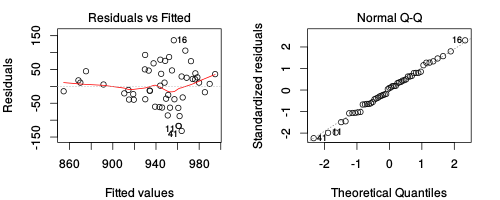
\includegraphics[width=.9\linewidth]{images/regressionsAssumptions1.png}

\end{block} \end{columns}
\end{frame}

\begin{frame}[fragile,label=sec-2-7]{Comparing models}
 Do congressional voting patterns predict SAT scores over and above expense? Fit two models and compare them:
\vspace{-.5em}
\begin{columns}
\column{.95\linewidth}
\begin{block}{}
\begin{minted}[linenos=false, fontsize=\footnotesize]{rconsole}
> # fit another model, adding house and senate as predictors
> sat.voting.mod <-  lm(csat ~ expense + house + senate,
+                       data = na.omit(states.data))
> sat.mod <- update(sat.mod, data=na.omit(states.data))
> # compare using the anova() function
> anova(sat.mod, sat.voting.mod)
Analysis of Variance Table

Model 1: csat ~ expense
Model 2: csat ~ expense + house + senate
  Res.Df    RSS Df Sum of Sq    F Pr(>F)
1     46 169050                         
2     44 149284  2     19766 2.91  0.065
> coef(summary(sat.voting.mod))
             Estimate Std. Error t value Pr(>|t|)
(Intercept) 1082.9344   38.63381   28.03 1.07e-29
expense       -0.0187    0.00969   -1.93 6.00e-02
house         -1.4424    0.60048   -2.40 2.06e-02
senate         0.4982    0.51356    0.97 3.37e-01
>
\end{minted}
\end{block}
\end{columns}
\vspace{.5em}
\end{frame}


\begin{frame}[fragile,label=sec-2-8]{Exercise 0: least squares regression}
 Use the \emph{states.rds} data set. Fit a model predicting  energy consumed per capita (energy) from the percentage of residents living in metropolitan areas (metro). Be sure to 
\begin{enumerate}
\item Examine/plot the data before fitting the model
\item Print and interpret the model \texttt{summary}
\item \texttt{plot} the model to look for deviations from modeling assumptions
\end{enumerate}

Select one or more additional predictors to add to your model and repeat steps 1-3. Is this model significantly better than the model with \emph{metro} as the only predictor?
\end{frame}

\section{Interactions and factors}
\label{sec-3}

\begin{frame}[fragile,label=sec-3-1]{Modeling interactions}
 Interactions allow us assess the extent to which the association between one predictor and the outcome depends on a second predictor. For example: Does the association between expense and SAT scores depend on the median income in the state?
\vspace{-.5em}
\begin{columns}
\column{.95\linewidth}
\begin{block}{}
\begin{minted}[linenos=false, fontsize=\footnotesize]{rconsole}
>   #Add the interaction to the model
> sat.expense.by.percent <- lm(csat ~ expense*income,
+                              data=states.data) 
> #Show the results
>   coef(summary(sat.expense.by.percent)) # show regression coefficients table
                 Estimate Std. Error t value       Pr(>|t|)
(Intercept)    1380.36423 172.086252    8.02 0.000000000237
expense          -0.06384   0.032701   -1.95 0.056878369245
income          -10.49785   4.991463   -2.10 0.040832525071
expense:income    0.00138   0.000864    1.60 0.115539488253
>
\end{minted}
\end{block}
\end{columns}
\vspace{.5em}
\end{frame}

\begin{frame}[fragile,label=sec-3-2]{Regression with categorical predictors}
 Let's try to predict SAT scores from region, a categorical variable. Note that you must make sure R does not think your categorical variable is numeric. 
\vspace{-.5em}
\begin{columns}
\column{.95\linewidth}
\begin{block}{}
\begin{minted}[linenos=false, fontsize=\footnotesize]{rconsole}
> # make sure R knows region is categorical
> str(states.data$region)
 Factor w/ 4 levels "West","N. East",..: 3 1 1 3 1 1 2 3 NA 3 ...
> states.data$region <- factor(states.data$region)
> #Add region to the model
> sat.region <- lm(csat ~ region,
+                  data=states.data) 
> #Show the results
> coef(summary(sat.region)) # show regression coefficients table
              Estimate Std. Error t value Pr(>|t|)
(Intercept)      946.3       14.8  63.958 1.35e-46
regionN. East    -56.8       23.1  -2.453 1.80e-02
regionSouth      -16.3       19.9  -0.819 4.17e-01
regionMidwest     63.8       21.4   2.986 4.51e-03
> anova(sat.region) # show ANOVA table
Analysis of Variance Table

Response: csat
          Df Sum Sq Mean Sq F value   Pr(>F)
region     3  82049   27350    9.61 0.000049
Residuals 46 130912    2846                 
>
\end{minted}
\end{block}
\end{columns}
\vspace{.5em}

Again, \alert{make sure to tell R which variables are categorical by converting them to factors!}
\end{frame}

\begin{frame}[fragile,label=sec-3-3]{Setting factor reference groups and contrasts}
 In the previous example we use the default contrasts for region. The default in R is treatment contrasts, with the first level as the reference. We can change the reference group or use another coding scheme using the \texttt{C} function.

\vspace{-.5em}
\begin{columns}
\column{.95\linewidth}
\begin{block}{}
\begin{minted}[linenos=false, fontsize=\footnotesize]{rconsole}
> # print default contrasts
> contrasts(states.data$region)
        N. East South Midwest
West          0     0       0
N. East       1     0       0
South         0     1       0
Midwest       0     0       1
> # change the reference group
> coef(summary(lm(csat ~ C(region, base=4),
+                 data=states.data)))
                     Estimate Std. Error t value Pr(>|t|)
(Intercept)            1010.1       15.4   65.59 4.30e-47
C(region, base = 4)1    -63.8       21.4   -2.99 4.51e-03
C(region, base = 4)2   -120.5       23.5   -5.12 5.80e-06
C(region, base = 4)3    -80.1       20.4   -3.93 2.83e-04
> # change the coding scheme
> coef(summary(lm(csat ~ C(region, contr.helmert),
+                 data=states.data)))
                          Estimate Std. Error t value Pr(>|t|)
(Intercept)                 943.99       7.71 122.498 1.69e-59
C(region, contr.helmert)1   -28.38      11.57  -2.453 1.80e-02
C(region, contr.helmert)2     4.02       5.88   0.684 4.98e-01
C(region, contr.helmert)3    22.03       4.45   4.955 1.02e-05
>
\end{minted}
\end{block}
\end{columns}
\vspace{.5em}

See also \texttt{?contrasts}, \texttt{?contr.treatment}, and \texttt{?relevel}.
\end{frame}

\begin{frame}[label=sec-3-4]{Exercise 1: interactions and factors}
Use the states data set.

\begin{enumerate}
\item Add on to the regression equation that you created in exercise 1 by generating an interaction term and testing the interaction.

\item Try adding region to the model. Are there significant differences across the four regions?
\end{enumerate}
\end{frame}

\section{Regression with binary outcomes}
\label{sec-4}

\begin{frame}[fragile,label=sec-4-1]{Logistic regression}
 This far we have used the \texttt{lm} function to fit our regression models. \texttt{lm} is great, but limited--in particular it only fits models for continuous dependent variables. For categorical dependent variables we can use the \texttt{glm()} function.

For these models we will use a different dataset, drawn from the National Health Interview Survey. From the \href{http://www.cdc.gov/nchs/nhis.htm}{CDC website}:

\begin{quote}
The National Health Interview Survey (NHIS) has monitored the health of the nation since 1957. NHIS data on a broad range of health topics are collected through personal household interviews. For over 50 years, the U.S. Census Bureau has been the data collection agent for the National Health Interview Survey. Survey results have been instrumental in providing data to track health status, health care access, and progress toward achieving national health objectives.
\end{quote}

Load the National Health Interview Survey data:

\vspace{-.5em}
\begin{columns}
\column{.95\linewidth}
\begin{block}{}
\begin{minted}[linenos=false, fontsize=\footnotesize]{rconsole}
> NH11 <- readRDS("dataSets/NatHealth2011.rds")
> labs <- attributes(NH11)$labels
>
\end{minted}
\end{block}
\end{columns}
\vspace{.5em}
\end{frame}

\begin{frame}[fragile,label=sec-4-2]{Logistic regression example}
 Let's predict the probability of being diagnosed with hypertension based on age, sex, sleep, and bmi

\vspace{-.5em}
\begin{columns}
\column{.95\linewidth}
\begin{block}{}
\begin{minted}[linenos=false, fontsize=\footnotesize]{rconsole}
> str(NH11$hypev) # check stucture of hypev
 Factor w/ 5 levels "1 Yes","2 No",..: 2 2 1 2 2 1 2 2 1 2 ...
> levels(NH11$hypev) # check levels of hypev
[1] "1 Yes"             "2 No"              "7 Refused"        
[4] "8 Not ascertained" "9 Don't know"     
> # collapse all missing values to NA
> NH11$hypev <- factor(NH11$hypev, levels=c("2 No", "1 Yes"))
> # run our regression model
> hyp.out <- glm(hypev~age_p+sex+sleep+bmi,
+               data=NH11, family="binomial")
> coef(summary(hyp.out))
            Estimate Std. Error z value Pr(>|z|)
(Intercept) -4.26947   0.056495  -75.57 0.00e+00
age_p        0.06070   0.000823   73.78 0.00e+00
sex2 Female -0.14403   0.026798   -5.37 7.68e-08
sleep       -0.00704   0.001640   -4.29 1.78e-05
bmi          0.01857   0.000951   19.53 6.49e-85
>
\end{minted}
\end{block}
\end{columns}
\vspace{.5em}
\end{frame}

\begin{frame}[fragile,label=sec-4-3]{Logistic regression coefficients}
 Generalized linear models use link functions, so raw coefficients are difficult to interpret. For example, the age coefficient of .06 in the previous model tells us that for every one unit increase in age, the log odds of hypertension diagnosis increases by 0.06. Since most of us are not used to thinking in log odds this is not too helpful!

One solution is to transform the coefficients to make them easier to interpret

\vspace{-.5em}
\begin{columns}
\column{.95\linewidth}
\begin{block}{}
\begin{minted}[linenos=false, fontsize=\footnotesize]{rconsole}
> hyp.out.tab <- coef(summary(hyp.out))
> hyp.out.tab[, "Estimate"] <- exp(coef(hyp.out))
> hyp.out.tab
            Estimate Std. Error z value Pr(>|z|)
(Intercept)    0.014   0.056495  -75.57 0.00e+00
age_p          1.063   0.000823   73.78 0.00e+00
sex2 Female    0.866   0.026798   -5.37 7.68e-08
sleep          0.993   0.001640   -4.29 1.78e-05
bmi            1.019   0.000951   19.53 6.49e-85
>
\end{minted}
\end{block}
\end{columns}
\vspace{.5em}
\end{frame}

\begin{frame}[fragile,label=sec-4-4]{Generating predicted values}
 In addition to transforming the log-odds produced by \texttt{glm} to odds, we can use the \texttt{predict()} function to make direct statements about the predictors in our model. For example, we can ask "How much more likely is a 63 year old female to have hypertension compared to a 33 year old female?".

\vspace{-.5em}
\begin{columns}
\column{.95\linewidth}
\begin{block}{}
\begin{minted}[linenos=false, fontsize=\footnotesize]{rconsole}
> # Create a dataset with predictors set at desired levels
> predDat <- with(NH11,
+                 expand.grid(age_p = c(33, 63),
+                             sex = "2 Female",
+                             bmi = mean(bmi, na.rm = TRUE),
+                             sleep = mean(sleep, na.rm = TRUE)))
> # predict hypertension at those levels
> cbind(predDat, predict(hyp.out, type = "response",
+                        se.fit = TRUE, interval="confidence",
+                        newdata = predDat))
  age_p      sex  bmi sleep   fit  se.fit residual.scale
1    33 2 Female 29.9  7.86 0.129 0.00285              1
2    63 2 Female 29.9  7.86 0.478 0.00482              1
>
\end{minted}
\end{block}
\end{columns}
\vspace{.5em}

This tells us that a 33 year old female has a 13\% probability of having been diagnosed with hypertension, while and 63 year old female has a 48\% probability of having been diagnosed.
\end{frame}

\begin{frame}[fragile,label=sec-4-5]{Packages for  computing and graphing predicted values}
 Instead of doing all this ourselves, we can use the effects package to compute quantities of interest for us (cf. the Zelig package).

\begin{columns} \column{.9\textwidth} \begin{block}{}
\begin{minted}[fontsize=\scriptsize]{r}
library(effects)
plot(allEffects(hyp.out))
\end{minted}

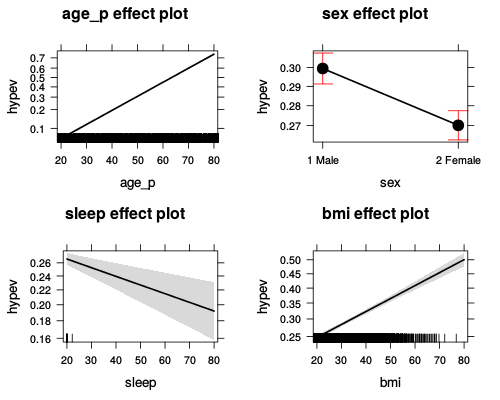
\includegraphics[width=.9\linewidth]{images/effects1.png}
\end{block} \end{columns}
\end{frame}



\begin{frame}[label=sec-4-6]{Exercise 2: logistic regression}
Use the NH11 data set that we loaded earlier.

\begin{enumerate}
\item Use glm  to conduct a logistic regression to predict ever worked (everwrk) using age (age$_{\text{p}}$) and marital status (r$_{\text{maritl}}$).
\item Predict the probability of working for each level of marital status.
\end{enumerate}

Note that the data is not perfectly clean and ready to be modeled. You will need to clean up at least some of the variables before fitting the model.
\end{frame}


\section{Multilevel Modeling}
\label{sec-5}


\begin{frame}[fragile,label=sec-5-1]{Multilevel modeling overview}
 \begin{itemize}
\item Multi-level (AKA hierarchical) models are a type of mixed-effects models
\item Used to model variation due to group membership where the goal is to generalize to a population of groups
\item Can model different intercepts and/or slopes for each group
\item Mixed-effecs models include two types of predictors: fixed-effects and random effects
\begin{description}
\item[{Fixed-effects}] observed levels are of direct interest (.e.g, sex, political party\ldots{})
\item[{Random-effects}] observed levels not of direct interest: goal is to make inferences to a population represented by observed levels
\end{description}
\item In R the lme4 package is the most popular for mixed effects models
\begin{itemize}
\item Use the \texttt{lmer} function for liner mixed models, \texttt{glmer} for generalized mixed models
\end{itemize}
\end{itemize}

\vspace{-.5em}
\begin{columns}
\column{.95\linewidth}
\begin{block}{}
\begin{minted}[linenos=false, fontsize=\footnotesize]{rconsole}
> library(lme4)
>
\end{minted}
\end{block}
\end{columns}
\vspace{.5em}
\end{frame}


\begin{frame}[fragile,label=sec-5-2]{The Exam data}
 The Exam data set contans exam scores of 4,059 students from 65 schools in Inner London. The variable names are as follows:

\begin{description}
\item[{school}] School ID - a factor.
\item[{normexam}] Normalized exam score.
\item[{schgend}] School gender - a factor.  Levels are 'mixed', 'boys', and 'girls'.
\item[{schavg}] School average of intake score.
\item[{vr}] Student level Verbal Reasoning (VR) score band at intake - a factor.  Levels are 'bottom 25\%', 'mid 50\%', and 'top 25\%'.
\item[{intake}] Band of student's intake score - a factor.  Levels are 'bottom 25\%', 'mid 50\%' and 'top 25\%'./
\item[{standLRT}] Standardised LR test score.
\item[{sex}] Sex of the student - levels are 'F' and 'M'.
\item[{type}] School type - levels are 'Mxd' and 'Sngl'.
\item[{student}] Student id (within school) - a factor
\end{description}

\vspace{-.5em}
\begin{columns}
\column{.95\linewidth}
\begin{block}{}
\begin{minted}[linenos=false, fontsize=\footnotesize]{rconsole}
> Exam <- readRDS("dataSets/Exam.rds")
>
\end{minted}
\end{block}
\end{columns}
\vspace{.5em}
\end{frame}


\begin{frame}[fragile,label=sec-5-3]{The null model and ICC}
 As a preliminary step it is often useful to partition the variance in the dependent variable into the various levels. This can be accomplished by running a null model (i.e., a model with a random effects grouping structure, but no fixed-effects predictors).

\vspace{-.5em}
\begin{columns}
\column{.95\linewidth}
\begin{block}{}
\begin{minted}[linenos=false, fontsize=\footnotesize]{rconsole}
> # null model, grouping by school but not fixed effects.
> Norm1 <-lmer(normexam ~ 1 + (1|school),
+               data=Exam, REML = FALSE)
> summary(Norm1)
Linear mixed model fit by maximum likelihood  ['lmerMod']
Formula: normexam ~ 1 + (1 | school)
   Data: Exam

     AIC      BIC   logLik deviance df.resid 
   10826    10844    -5410    10820     3984 

Scaled residuals: 
   Min     1Q Median     3Q    Max 
-3.902 -0.646  0.003  0.698  3.636 

Random effects:
 Groups   Name        Variance Std.Dev.
 school   (Intercept) 0.169    0.412   
 Residual             0.848    0.921   
Number of obs: 3987, groups:  school, 65

Fixed effects:
            Estimate Std. Error t value
(Intercept)  -0.0141     0.0538   -0.26
>
\end{minted}
\end{block}
\end{columns}
\vspace{.5em}

The is .169/(.169 + .848) = .17: 17\% of the variance is at the school level.
\end{frame}
\begin{frame}[fragile,label=sec-5-4]{Adding fixed-effects predictors}
 Predict exam scores from student's standardized tests scores

\vspace{-.5em}
\begin{columns}
\column{.95\linewidth}
\begin{block}{}
\begin{minted}[linenos=false, fontsize=\footnotesize]{rconsole}
> Norm2 <-lmer(normexam~standLRT + (1|school),
+              data=Exam,
+              REML = FALSE) 
> summary(Norm2) 
Linear mixed model fit by maximum likelihood  ['lmerMod']
Formula: normexam ~ standLRT + (1 | school)
   Data: Exam

     AIC      BIC   logLik deviance df.resid 
    9143     9168    -4568     9135     3954 

Scaled residuals: 
   Min     1Q Median     3Q    Max 
-3.700 -0.625  0.024  0.678  3.262 

Random effects:
 Groups   Name        Variance Std.Dev.
 school   (Intercept) 0.0919   0.303   
 Residual             0.5670   0.753   
Number of obs: 3958, groups:  school, 65

Fixed effects:
            Estimate Std. Error t value
(Intercept)  0.00121    0.04004     0.0
standLRT     0.56559    0.01265    44.7

Correlation of Fixed Effects:
         (Intr)
standLRT 0.007 
>
\end{minted}
\end{block}
\end{columns}
\vspace{.5em}
\end{frame}


\begin{frame}[fragile,label=sec-5-5]{Multiple degree of freedom comparisons}
 As with \texttt{lm} and \texttt{glm} models, you can compare the two \texttt{lmer} models using the \texttt{anova} function.

\vspace{-.5em}
\begin{columns}
\column{.95\linewidth}
\begin{block}{}
\begin{minted}[linenos=false, fontsize=\footnotesize]{rconsole}
> anova(Norm1, Norm2)
Data: Exam
Models:
Norm1: normexam ~ 1 + (1 | school)
Norm2: normexam ~ standLRT + (1 | school)
      Df   AIC   BIC logLik deviance Chisq Chi Df Pr(>Chisq)
Norm1  3 10826 10844  -5410    10820                        
Norm2  4  9143  9169  -4568     9135  1684      1     <2e-16
>
\end{minted}
\end{block}
\end{columns}
\vspace{.5em}
\end{frame}


\begin{frame}[fragile,label=sec-5-6]{Random slopes}
 Add a random effect of students' standardized test scores as well. Now in addition to estimating the distribution of intercepts across schools, we also estimate the distribution of the slope of exam on standardized test.

\vspace{-.5em}
\begin{columns}
\column{.95\linewidth}
\begin{block}{}
\begin{minted}[linenos=false, fontsize=\footnotesize]{rconsole}
> Norm3 <- lmer(normexam~standLRT + (standLRT|school), data=Exam,
+                REML = FALSE) 
> summary(Norm3) 
Linear mixed model fit by maximum likelihood  ['lmerMod']
Formula: normexam ~ standLRT + (standLRT | school)
   Data: Exam

     AIC      BIC   logLik deviance df.resid 
    9108     9146    -4548     9096     3952 

Scaled residuals: 
   Min     1Q Median     3Q    Max 
-3.813 -0.634  0.033  0.673  3.452 

Random effects:
 Groups   Name        Variance Std.Dev. Corr
 school   (Intercept) 0.0899   0.300        
          standLRT    0.0141   0.119    0.51
 Residual             0.5552   0.745        
Number of obs: 3958, groups:  school, 65

Fixed effects:
            Estimate Std. Error t value
(Intercept)  -0.0122     0.0397   -0.31
standLRT      0.5586     0.0199   28.08

Correlation of Fixed Effects:
         (Intr)
standLRT 0.371 
>
\end{minted}
\end{block}
\end{columns}
\vspace{.5em}
\end{frame}

\begin{frame}[fragile,label=sec-5-7]{Test the significance of the random slope}
 To test the significance of a random slope just compare models with and without the random slope term 

\vspace{-.5em}
\begin{columns}
\column{.95\linewidth}
\begin{block}{}
\begin{minted}[linenos=false, fontsize=\footnotesize]{rconsole}
> anova(Norm2, Norm3) 
Data: Exam
Models:
Norm2: normexam ~ standLRT + (1 | school)
Norm3: normexam ~ standLRT + (standLRT | school)
      Df  AIC  BIC logLik deviance Chisq Chi Df   Pr(>Chisq)
Norm2  4 9143 9169  -4568     9135                          
Norm3  6 9108 9146  -4548     9096    39      2 0.0000000035
>
\end{minted}
\end{block}
\end{columns}
\vspace{.5em}
\end{frame}


\begin{frame}[fragile,label=sec-5-8]{Exercise 3: multilevel modeling}
 Use the dataset, bh1996:
\begin{minted}[fontsize=\scriptsize]{r}
data(bh1996, package="multilevel")
\end{minted}

From the data documentation:
\begin{quote}
Variables are Cohesion (COHES), Leadership Climate (LEAD),
Well-Being (WBEING) and Work Hours (HRS).  Each of these variables
has two variants - a group mean version that replicates each group
mean for every individual, and a within-group version where the
group mean is subtracted from each individual response.  The group
mean version is designated with a G. (e.g., G.HRS), and the
within-group version is designated with a W. (e.g., W.HRS).
\end{quote}

\begin{enumerate}
\item Create a null model predicting wellbeing ("WBEING")
\item Calculate the ICC for your null model
\item Run a second multi-level model that adds two individual-level predictors, average number of hours worked ("HRS") and leadership skills ("LEAD") to the model and interpret your output.
\item Now, add a random effect of average number of hours worked ("HRS") to the model and interpret your output.  Test the significance of this random term.
\end{enumerate}
\end{frame}


\section{Exercise solutions\hfill{}\textsc{prototype}}
\label{sec-6}

\begin{frame}[fragile,label=sec-6-1]{Exercise 0 prototype}
 Use the \emph{states.rds} data set. 
\begin{minted}[fontsize=\scriptsize]{r}
states <- readRDS("dataSets/states.rds")
\end{minted}

Fit a model predicting  energy consumed per capita (energy) from the percentage of residents living in metropolitan areas (metro). Be sure to 
\begin{enumerate}
\setcounter{enumi}{0}
\item Examine/plot the data before fitting the model
\end{enumerate}
\begin{minted}[fontsize=\scriptsize]{r}
states.en.met <- subset(states, select = c("metro", "energy"))
summary(states.en.met)
plot(states.en.met)
cor(states.en.met, use="pairwise")
\end{minted}

\begin{enumerate}
\setcounter{enumi}{1}
\item Print and interpret the model \texttt{summary}
\end{enumerate}
\begin{minted}[fontsize=\scriptsize]{r}
mod.en.met <- lm(energy ~ metro, data = states)
summary(mod.en.met)
\end{minted}

\begin{enumerate}
\setcounter{enumi}{2}
\item \texttt{plot} the model to look for deviations from modeling assumptions
\end{enumerate}
\begin{minted}[fontsize=\scriptsize]{r}
plot(mod.en.met)
\end{minted}

Select one or more additional predictors to add to your model and repeat steps 1-3. Is this model significantly better than the model with \emph{metro} as the only predictor?
\begin{minted}[fontsize=\scriptsize]{r}
states.en.met.pop.wst <- subset(states, select = c("energy", "metro", "pop", "waste"))
summary(states.en.met.pop.wst)
plot(states.en.met.pop.wst)
cor(states.en.met.pop.wst, use = "pairwise")
mod.en.met.pop.waste <- lm(energy ~ metro + pop + waste, data = states)
summary(mod.en.met.pop.waste)
anova(mod.en.met, mod.en.met.pop.waste)
\end{minted}
\end{frame}

\begin{frame}[fragile,label=sec-6-2]{Exercise 1: prototype}
 Use the states data set.

\begin{enumerate}
\item Add on to the regression equation that you created in exercise 1 by generating an interaction term and testing the interaction.
\end{enumerate}
\begin{minted}[fontsize=\scriptsize]{r}
mod.en.metro.by.waste <- lm(energy ~ metro * waste, data = states)
\end{minted}

\begin{enumerate}
\item Try adding a region to the model. Are there significant differences across the four regions?
\end{enumerate}
\begin{minted}[fontsize=\scriptsize]{r}
mod.en.region <- lm(energy ~ metro * waste + region, data = states)
anova(mod.en.region)
\end{minted}
\end{frame}

\begin{frame}[fragile,label=sec-6-3]{Exercise 2 prototype}
 Use the NH11 data set that we loaded earlier. Note that the data is not perfectly clean and ready to be modeled. You will need to clean up at least some of the variables before fitting the model.

\begin{enumerate}
\setcounter{enumi}{0}
\item Use glm  to conduct a logistic regression to predict ever worked (everwrk) using age (age$_{\text{p}}$) and marital status (r$_{\text{maritl}}$).
\end{enumerate}
\begin{minted}[fontsize=\scriptsize]{r}
nh11.wrk.age.mar <- subset(NH11, select = c("everwrk", "age_p", "r_maritl"))
summary(nh11.wrk.age.mar)
NH11 <- transform(NH11,
                  everwrk = factor(everwrk,
                      levels = c("1 Yes", "2 No")),
                  r_maritl = droplevels(r_maritl))

mod.wk.age.mar <- glm(everwrk ~ age_p + r_maritl, data = NH11,
                      family = "binomial")

summary(mod.wk.age.mar)
\end{minted}

\begin{enumerate}
\setcounter{enumi}{1}
\item Predict the probability of working for each level of marital status.
\end{enumerate}
\begin{minted}[fontsize=\scriptsize]{r}
library(effects)
data.frame(Effect("r_maritl", mod.wk.age.mar))
\end{minted}
\end{frame}



\begin{frame}[fragile,label=sec-6-4]{Exercise 3 prototype}
 Use the dataset, bh1996:
\begin{minted}[fontsize=\scriptsize]{r}
data(bh1996, package="multilevel")
\end{minted}

From the data documentation:
\begin{quote}
Variables are Cohesion (COHES), Leadership Climate (LEAD),
Well-Being (WBEING) and Work Hours (HRS).  Each of these variables
has two variants - a group mean version that replicates each group
mean for every individual, and a within-group version where the
group mean is subtracted from each individual response.  The group
mean version is designated with a G. (e.g., G.HRS), and the
within-group version is designated with a W. (e.g., W.HRS).
\end{quote}
Note that the group identifier is named "GRP".
\begin{enumerate}
\setcounter{enumi}{0}
\item Create a null model predicting wellbeing ("WBEING")
\end{enumerate}
\begin{minted}[fontsize=\scriptsize]{r}
library(lme4)
mod.grp0 <- lmer(WBEING ~ 1 + (1 | GRP), data = bh1996)
summary(mod.grp0)
\end{minted}
=> library(lme4)
> mod.grp0 <- lmer(WBEING \textasciitilde{} 1 + (1 | GRP), data = bh1996)
> summary(mod.grp0)
Linear mixed model fit by REML ['lmerMod']
Formula: WBEING \textasciitilde{} 1 + (1 | GRP)
   Data: bh1996

REML criterion at convergence: 19347

Scaled residuals: 
   Min     1Q Median     3Q    Max 
-3.322 -0.648  0.031  0.718  2.667 

Random effects:
 Groups   Name        Variance Std.Dev.
 GRP      (Intercept) 0.0358   0.189   
 Residual             0.7895   0.889   
Number of obs: 7382, groups:  GRP, 99

Fixed effects:
            Estimate Std. Error t value
(Intercept)   2.7743     0.0222     125
> 
=2. [@2] Calculate the ICC for your null model
 \verb~ICC = .0358/(.0358 + .7895) = .04~
\begin{enumerate}
\setcounter{enumi}{2}
\item Run a second multi-level model that adds two individual-level predictors, average number of hours worked ("HRS") and leadership skills ("LEAD") to the model and interpret your output.
\end{enumerate}
\begin{minted}[fontsize=\scriptsize]{r}
mod.grp1 <- lmer(WBEING ~ HRS + LEAD + (1 | GRP), data = bh1996)
summary(mod.grp1)
\end{minted}

\begin{enumerate}
\setcounter{enumi}{3}
\item Now, add a random effect of average number of hours worked ("HRS") to the model and interpret your output.  Test the significance of this random term.
\end{enumerate}
\begin{minted}[fontsize=\scriptsize]{r}
mod.grp2 <- lmer(WBEING ~ HRS + LEAD + (1 + HRS | GRP), data = bh1996)
anova(mod.grp1, mod.grp2)
\end{minted}
\end{frame}


\section{Wrap-up}
\label{sec-7}

\begin{frame}[label=sec-7-1]{Help us make this workshop better!}
\begin{itemize}
\item Please take a moment to fill out a very short
\end{itemize}
feedback form 
\begin{itemize}
\item These workshops exist for you -- tell us what you need!
\item \url{http://tinyurl.com/RstatisticsFeedback}
\end{itemize}
\end{frame}


\begin{frame}[label=sec-7-2]{Additional resources}
\begin{itemize}
\item IQSS workshops: \url{http://projects.iq.harvard.edu/rtc/filter_by/workshops}
\item IQSS statistical consulting: \url{http://rtc.iq.harvard.edu}

\item Zelig
\begin{itemize}
\item Website: \url{http://gking.harvard.edu/zelig}
\item Documentation: \url{http://r.iq.harvard.edu/docs/zelig.pdf}
\end{itemize}
\item Ameila
\begin{itemize}
\item Website: \url{http://gking.harvard.edu/Amelia/}
\item Documetation: \url{http://r.iq.harvard.edu/docs/amelia/amelia.pdf}
\end{itemize}
\end{itemize}
\end{frame}
% Emacs 24.3.1 (Org mode 8.2.7c)
\end{document}